\documentclass{standalone}
\usepackage{tikz}
\usetikzlibrary{calc}

\begin{document}

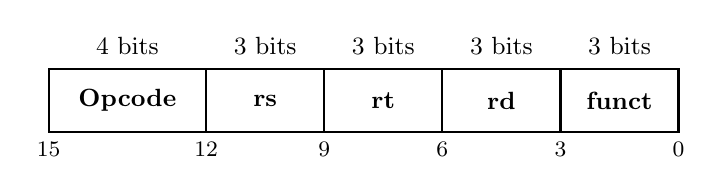
\begin{tikzpicture}[
    font=\small,
    box/.style={draw, thick, minimum height=0.8cm, outer sep=0pt, anchor=west}
]

    % --- Top Width Labels ---
    \node at (1.0, 0.7) {4 bits};
    \node at (2.75, 0.7) {3 bits};
    \node at (4.25, 0.7) {3 bits};
    \node at (5.75, 0.7) {3 bits};
    \node at (7.25, 0.7) {3 bits};

    % --- Main Instruction Box ---
    \node[box, minimum width=2.0cm] (b1) at (0,0) {\textbf{Opcode}};
    \node[box, minimum width=1.5cm] (b2) at (b1.east) {\textbf{rs}};
    \node[box, minimum width=1.5cm] (b3) at (b2.east) {\textbf{rt}};
    \node[box, minimum width=1.5cm] (b4) at (b3.east) {\textbf{rd}};
    \node[box, minimum width=1.5cm] (b5) at (b4.east) {\textbf{funct}};

    % --- Bit Indices (With significant space below the box) ---
    % yshift=-0.4cm creates a clear "breathing" gap between the line and the number
    \begin{scope}[every node/.style={font=\footnotesize, anchor=north, yshift=-0.4cm}]
        \node at (b1.west) {15};
        \node at (b1.east) {12};
        \node at (b2.east) {9};
        \node at (b3.east) {6};
        \node at (b4.east) {3};
        \node at (b5.east) {0};
    \end{scope}

\end{tikzpicture}
\end{document}